\documentclass{article}

\title{Fungible tokens: payment flows}
\subtitle{Payment flows for fungible tokens on the Internet Computer.}
\date{2022-09-21}
\modified{2022-09-21}

\keyword{ic}
\keyword{ledger}
\keyword{fi}

\begin{document}
\section{introduction}{Introduction}

In the previous article, \href{/posts/09-fungible-tokens-101.html}{Fungible tokens 101}, I introduced the concept of a ledger and various extensions that can help us solve practical problems.
In this article, we shall analyze a few \emph{payment flows}---protocols built on top of a ledger allowing clients to exchange tokens for a service---in the context of the \href{https://internetcomputer.org}{Internet Computer}.

\section{prerequisites}{Prerequisites}
\subsection{the-payment-scenario}{The payment scenario}

Abstract protocols can be dull and hard to comprehend, so let us model a specific payment scenario: me buying a new laptop online and paying for it in \sc{wxdr} (wrapped \href{https://en.wikipedia.org/wiki/Special_drawing_rights}{\sc{sdr}}) tokens locked in a ledger hosted on the Internet Computer.

I open the website of the hardware vendor I trust, select the configuration (the memory capacity, the number of cores, etc.) that suits my needs, fill in the shipment details, and go to the payment page.
I choose an option to pay in \sc{wxdr}.

In the rest of the article, we will fantasize about what the payment page can look like and how it can interact with the shop.

\subsection{participants}{Participants}

Each flow will involve the following participants:

\begin{tabular*}{l l}
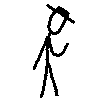
\includegraphics[grayscale]{/images/10-me.png} & \emph{Me}: a merry human sitting in front of a computer and ordering a new laptop. \\
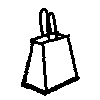
\includegraphics[grayscale]{/images/10-shop.png} & \emph{Shop}: an Internet Computer smart contract accepting orders. \\
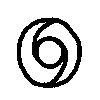
\includegraphics[grayscale]{/images/10-webpage.png} & \emph{Web page}: a spaghetti of markup, styling, and scripts serving the \emph{shop} UI. \\
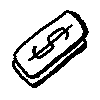
\includegraphics[grayscale]{/images/10-wallet.png} & \emph{Wallet}: a trusty hardware wallet device, such as \href{https://www.ledger.com/}{Ledger} or \href{https://trezor.io/}{Trezor}, with a corresponding UI for interacting with the ledger, such as \href{https://www.ledger.com/ledger-live}{Ledger Live}. A more sophisticated wallet can smoothen the UX, but the ideas remain the same. \\
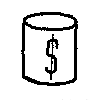
\includegraphics[grayscale]{/images/10-ledger.png} & \emph{Ledger}: an Internet Computer smart contract processing payments. \\
\end{tabular*}

\subsection{payment-phases}{Payment phases}

All the payment flows we will analyze have three phases:
\begin{enumerate}
  \item 
    \emph{The negotiation phase}.
    After I place my order and fill in the shipment details, the shop creates a unique order identifier, \emph{Invoice ID}.
    The \emph{web page} displays the payment details (e.g., as a \sc{qr} code of the request I need to sign) and instructions on how to proceed with the order.
  \item 
    \emph{The payment phase}.
    I use my \emph{wallet} to execute the transaction as instructed on the \emph{web page}.
    This phase is essentially the same in all flows; only the transaction type varies.
  \item 
    \emph{The notification phase}.
    The shop receives a payment notification for the Invoice ID, validates the payment, and updates the order status.
    The \emph{web page} displays an upbeat message, completing the flow.
\end{enumerate}

\section{invoice-account}{Invoice account}

The first payment flow we will analyze relies on the \href{/posts/09-fungible-tokens-101.html#subaccounts}{subaccounts} ledger feature.
The idea behind the flow is quite clever: the shop can use its subaccount identified by the \emph{Invoice ID} as a temporary ``cell'' for the payment.
I can transfer my tokens to this cell, and the shop can move tokens out because the cell belongs to the shop.

The happy case of the flow needs only one primitive from the ledger, the \code{transfer} method specified below.

\begin{code}[candid]
service : {
  \emph{// Transfers token \b{amount} from the account of the (implicit) \b{caller}}
  \emph{// to the account specified by the principal and the subaccount.}
  \emph{// Arguments:}
  \emph{//   \b{amount} - the token amount to transfer.}
  \emph{//   \b{from_subaccount} - the subaccount of the caller to transfer tokens from.}
  \emph{//   \b{to} - the receiver of the tokens.}
  \emph{//   \b{to_subaccount} - which subaccount of the receiver the tokens will land on.}
  \b{transfer}(record {
    amount : nat;
    from_subaccount : opt blob;
    to : principal;
    to_subaccount : opt blob;
  }) -> (TxReceipt);
}
\end{code}

The flow proceeds as follows:
\begin{enumerate}
  \item 
    In the negotiation phase, the webpage instructs me to transfer tokens to the shop's \emph{Invoice ID} subaccount and displays a big green ``Done'' button that I need to press after the payment succeeds.
  \item 
    In the payment phase, I use my wallet to execute the \code{transfer(\{ amount = Price, to = Shop, to_subaccount = InvoiceId\})} call on the ledger.
  \item 
    In the notification phase, I click on the ``Done'' button dispatching a notification to the \emph{shop} indicating that I paid the invoice (the webpage can remember the \emph{Invoice ID} on the client side, so I do not have to type it in).
    Upon receiving the notification, the shop attempts to transfer the amount from its \emph{Invoice ID} subaccount to its default account, calling \code{transfer(\{ amount = Price - Fee, from_subaccount = InvoiceID, to = Shop \})} on the ledger.
    If that final transfer succeeds, the order is complete.
\end{enumerate}

\begin{figure}[grayscale-diagram]
\marginnote{mn-invoice-account-seq}{
  A sequence diagram for the invoice account payment flow.
}
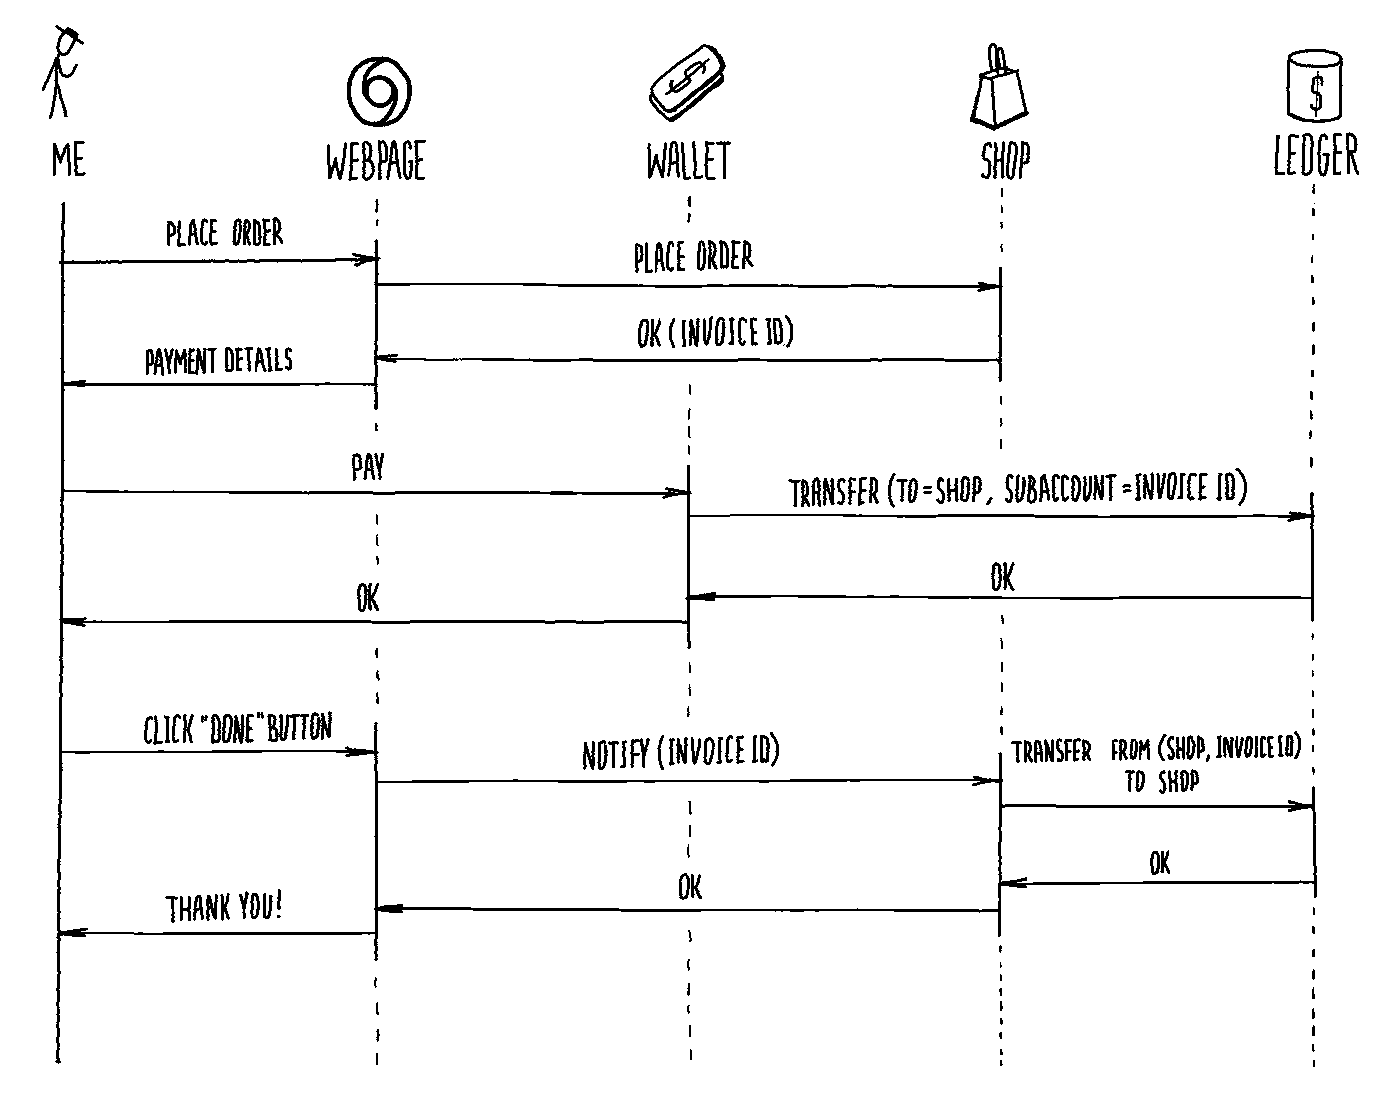
\includegraphics{/images/10-invoice-id-flow.png}
\end{figure}

The invoice account flow has a few interesting properties:
\begin{itemize}
  \item The ledger must process at least two messages: one transfer from me and another from the shop.
  \item Two transfers mean that the ledger charges \emph{two} fees for each flow: one from me and another from the shop.
  \item 
    The ledger needs to remember one additional \code{(principal, subaccount, amount)} tuple for the duration of the flow.
    The tuple occupies at least 70 bytes.
  \item The flow supports unlimited concurrency: I can make multiple payments to the same shop in parallel as long as each payment uses a unique invoice identifier.
  \item 
    The ledger implementation is straightforward: the subaccounts feature is the only requirement for the flow.
\end{itemize}

What happens if I transfer my \sc{wxdr}s but never click the ``Done'' button?
Or what if my browser loses network connection right before it sends the shop notification?
The shop will not receive any notifications, likely never making progress with my order.
One strategy that the shop could use to improve the user experience in such cases is to monitor balances for unpaid invoices and complete transactions automatically if the notification does not arrive in a reasonable amount of time.

\section{approve-transfer-from}{Approve-transfer-from}

The approve-transfer-from pattern relies on the \href{/posts/09-fungible-tokens-101.html#approvals}{approvals} ledger feature, first appearing in the \href{https://ethereum.org/en/developers/docs/standards/tokens/erc-20/}{ERC-20} token standard.
The flow uses two new ledger primitives, \code{approve} and \code{transfer_from}, and involves three parties:
\begin{enumerate}
  \item The \emph{owner} holds tokens on the ledger. The owner can \emph{approve} transfers from its account to a \emph{delegate}.
  \item The \emph{delegate} can \emph{transfer} tokens \emph{from} the owner's account within the approved cap.
  \item The \emph{beneficiary} receives tokens from the delegate as if the owner sent them.
\end{enumerate}

In our \href{#payment-scenario}{scenario}, the delegate and the beneficiary are the same entity---the \emph{shop}.

We can capture the required ledger primitives in the following Candid interface:
\begin{code}[candid]
service : {
  \emph{// Entitles the \b{delegate} to spend at most the specified token \b{amount} on behalf}
  \emph{// of the (implicit) \b{caller}.}
  \emph{// Arguments:}
  \emph{//   \b{amount} - the cap on the amount the delegate can transfer from the caller's account.}
  \emph{//   \b{delegate} - the actor entitled to make payments on behalf of the caller.}
  \b{approve}(record {
    amount : nat;
    delegate : principal;
  }) -> ();

  \emph{// Transfers the specified token \b{amount} from the \b{owner} account to the}
  \emph{// specified account.}
  \emph{// Arguments:}
  \emph{//   \b{amount} - the token amount to transfer.}
  \emph{//   \b{owner} - the account to transfer tokens from.}
  \emph{//   \b{to} - the receiver of the tokens (the beneficiary).}
  \emph{//}
  \emph{// PRECONDITION: the \b{owner} has approved at least the \b{amount} to the (implicit) \b{caller}.}
  \emph{// POSTCONDITION: the caller's allowance decreases by the \b{amount}.}
  \b{transfer_from}(record {
    amount : nat;
    owner : principal;
    to : principal;
  }) -> (nat) query;
}
\end{code}

The flow proceeds as follows:
\begin{enumerate}
  \item 
    In the negotiation phase, the webpage instructs me to approve a transfer to the shop, displaying the shop's account.
    One difference from the \href{#invoice-account}{invoice account} flow is that the shop needs to know my wallet's address on the ledger to make a transfer on my behalf.
    The webpage displays a text field for my account and the familiar ``Done'' button.
  \item In the payment phase, I use my wallet to execute the \code{approve(\{to = Shop, amount = Price\})} call on the ledger.
  \item 
    In the notification phase, I paste my ledger address into the text field and press the button.
    Once the shop receives the notification with my address and the \emph{Invoice ID}, it executes \code{transfer_from(\{ amount = Price; owner = Wallet; to = Shop \})} call on the ledger.
    If that transfer is successful, the order is complete.
\end{enumerate}

\begin{figure}[grayscale-diagram]
\marginnote{mn-approve-transfer-from-seq}{
  A sequence diagram for the approve-transfer-from payment flow.
}
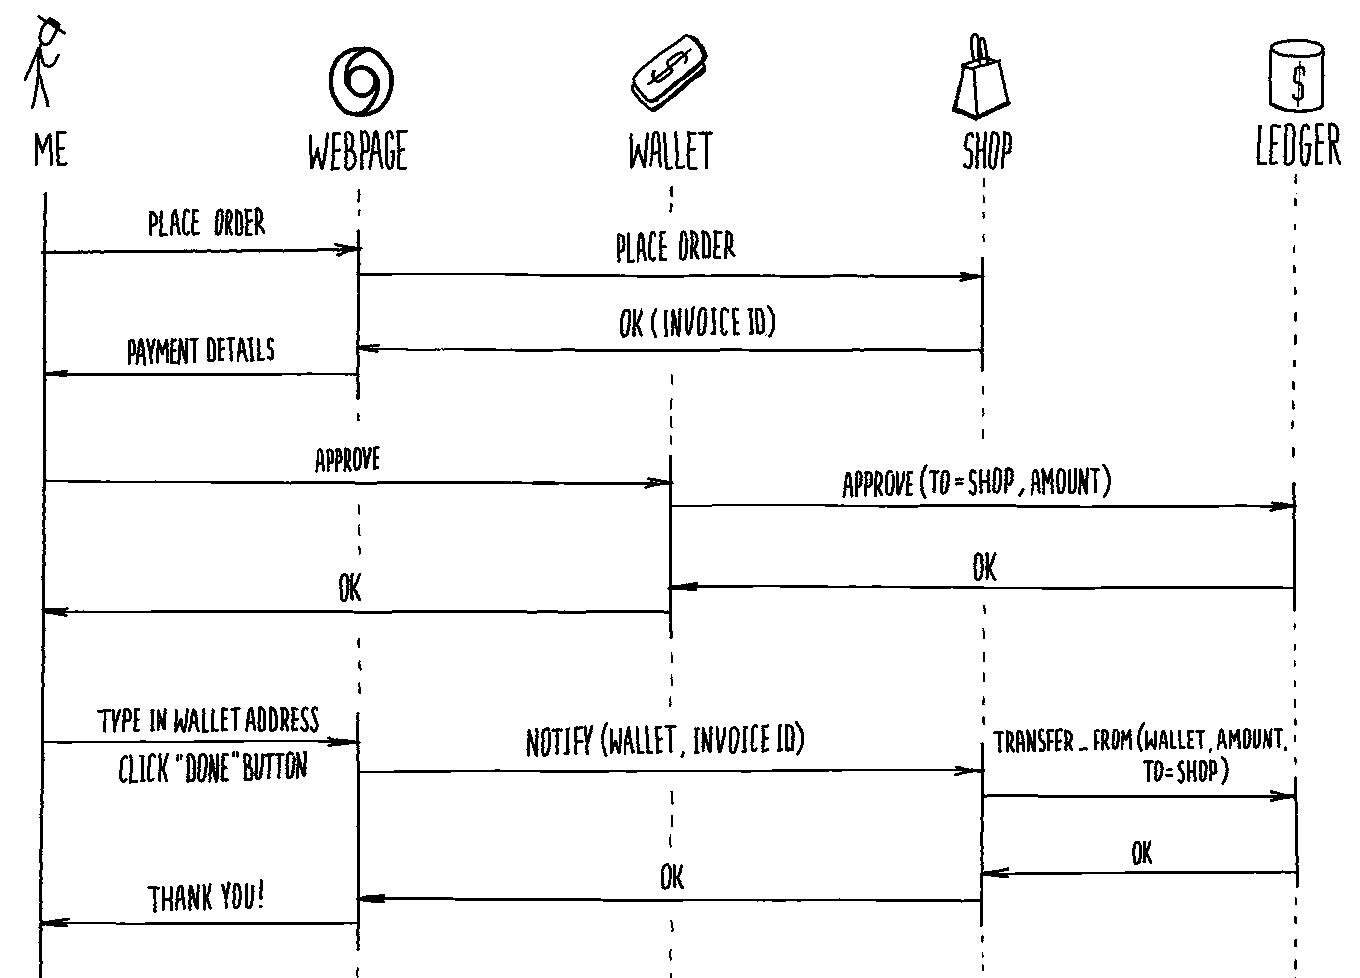
\includegraphics{/images/10-approve-flow.png}
\end{figure}

Let us see how this flow compares to the \href{#invoice-account}{invoice account} flow:
\begin{itemize}
  \item The ledger must process at least two messages: approval from the owner and a transfer from the shop.
  \item The ledger charges \emph{two} fees for each payment: one for my approval and another for the shop's transfer.
  \item 
    The ledger needs to remember one additional \code{(principal, principal, amount)} tuple for the duration of the flow.
    The tuple occupies at least 68 bytes.
  \item 
    The flow does not support concurrency: if I execute two payments to the same shop asynchronously, only one of the payments will likely succeed (the exact outcome depends on the message scheduling order).
  \item 
    The ledger needs to maintain a data structure to track allowances, adding complexity to the implementation.
  \item 
    I still have the tokens on my account if the shop never gets the notification due to a bug or a networking issue.
\end{itemize}

One strong side of the approve-transfer-from flow is that it supports recurring payments.
For example, if I were buying a subscription with monthly installments, I could have approved transfers for the entire year, allowing the shop to transfer from my account once a month.
Of course, I must trust the shop not to charge the whole yearly amount in one go.

\section{transfer-notify}{Transfer-notify}

Note that the failure of the frontend to send a notification is a prevalent error in the previous flows.
What if the ledger automatically delivered the notification to the receiver over the reliable channel that the Internet Computer provides?
That is the idea behind the transfer-notify flow.

There is one issue we need to sort out, however.
When we relied on the webpage to send the notification, we could include the \emph{Invoice ID} into the payload, making it possible for the shop to identify the relevant order.
If we ask the ledger to send the payment notification, we must pass the \emph{Invoice ID} in that message.
The common way to address this issue is to add the \code{memo} argument to the transfer arguments, allowing the caller to attach an arbitrary payload to the transaction details.

\begin{code}[candid]
service : {
  \emph{// Transfers token \b{amount} from the account of the (implicit) \b{caller}}
  \emph{// to the account specified by the principal.}
  \emph{// If the transfer is successful, sends a notification to the receiver.}
  \emph{// Arguments:}
  \emph{//   \b{amount} - the token amount to transfer.}
  \emph{//   \b{to} - the receiver of the tokens.}
  \emph{//   \b{memo} - an opaque identifier attached to the notification.}
  \b{transfer_notify}(record {
    amount : nat;
    to : principal;
    memo : opt blob;
  }) -> (TxReceipt);
}
\end{code}

The flow proceeds as follows:
\begin{enumerate}
  \item In the negotiation phase, the webpage displays the payment details and starts polling the shop for payment confirmation.
  \item In the payment phase, I use my wallet to execute the \code{transfer_notify(\{to = Shop, amount = Price, memo = InvoiceID\})} call on the ledger.
  \item 
    Once the transfer succeeds, the ledger notifies the shop about the payment, providing the amount and the \code{memo} containing the \emph{Invoice ID}.
    The shop consumes the notification and changes the order status.
    The next time the webpage polls the shop, the shop replies with a confirmation, and I see a positive message.
\end{enumerate}

\begin{figure}[grayscale-diagram]
\marginnote{mn-transfer-notify-seq}{
  A sequence diagram for the transfer-notify payment flow.
}
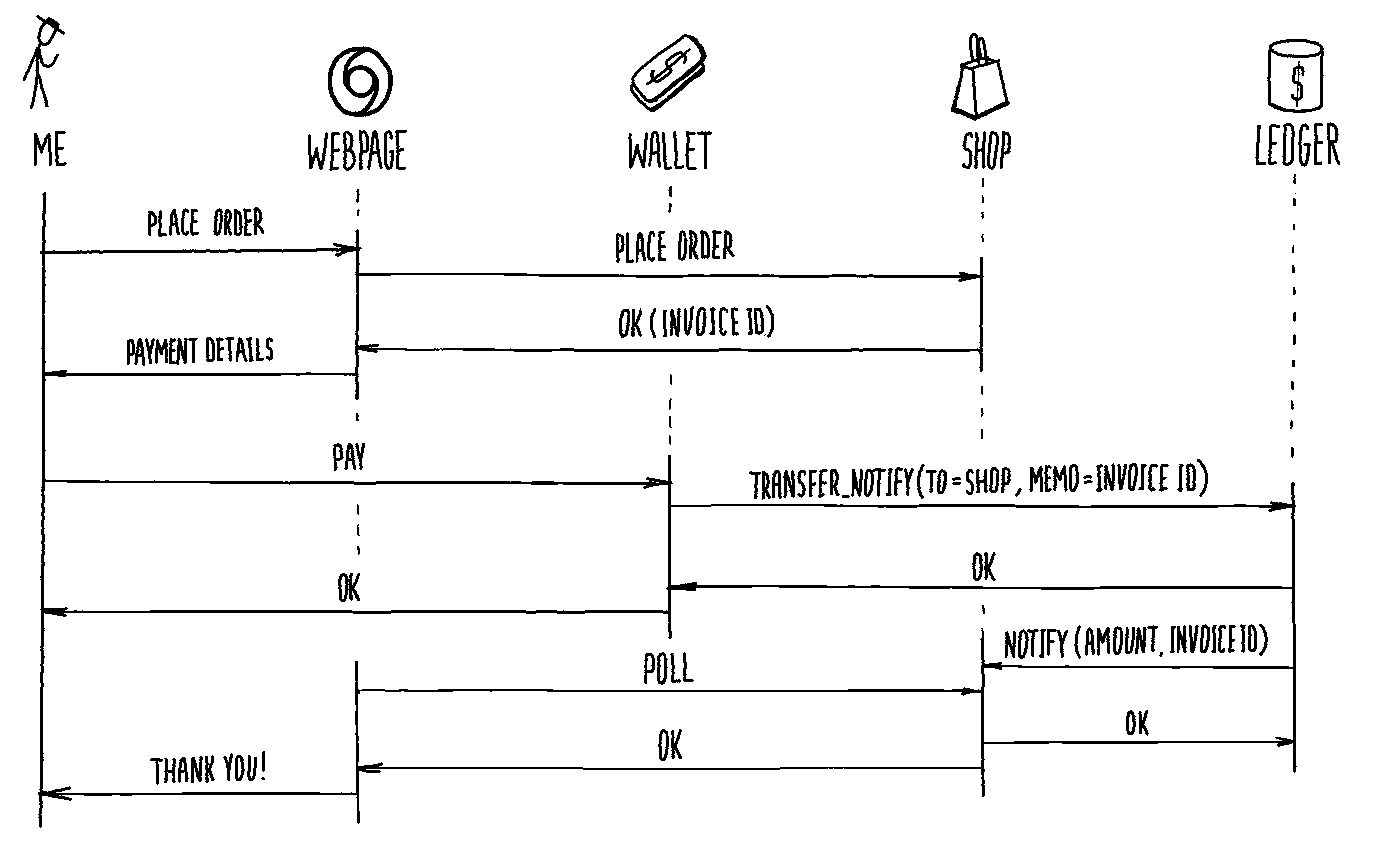
\includegraphics{/images/10-notify-flow.png}
\end{figure}

Let us check how this flow compares to the previous ones:
\begin{itemize}
  \item The ledger must process at least two messages: a transfer from the owner and a notification to the shop.
  \item 
    The ledger charges a combined fee for my transfer and notification.
    Whether the ledger charges two fees or gives a discount depends on the implementation.
    Let us assume that the ledger charges 1½ fees.
  \item 
    The ledger needs to hold a notification in memory until the flow completes.
    The notification must contain at least the payer principal, the memo (up to 32 bytes), and the amount, which amounts to at least 70 bytes per flow.
  \item The flow support unlimited concurrency.
  \item 
    The notification feature adds a lot of complexity to the ledger implementation.
    The ledger might need to deal with unresponsive destinations and implement a retry policy for delivering notifications.
  \item 
    The ledger sends the notification on-chain, making it very likely that the shop will receive the notification.
    Still, there is a possibility that the notification will not get through if the destination is overloaded.
\end{itemize}

\section{transfer-notify}{Transfer-fetch}

The transfer-fetch flow relies on the ability to request details of past transactions from the ledger.
After I transfer tokens to the shop, specifying the \emph{Invoice ID} as the transaction memo, the ledger issues a unique transaction identifier.
I can then pass this identifier to the shop as proof of my payment.
The shop can fetch transaction details directly from the ledger to validate the payment.
Below is the interface we expect from the ledger.

\begin{code}[candid]
service : {
  \emph{// Transfers token \b{amount} from the account of the (implicit) \b{caller}}
  \emph{// to the account specified by the principal.}
  \emph{// Returns a unique transaction identifier.}
  \emph{// Arguments:}
  \emph{//   \b{amount} - the token amount to transfer.}
  \emph{//   \b{to} - the receiver of the tokens.}
  \emph{//   \b{memo} - an opaque identifier attached to the transaction.}
  \b{transfer}(record {
    amount : nat;
    to : principal;
    memo : opt blob;
  }) -> (nat);

  \emph{// Retrieves details of the transaction with the specified identifier.}
  \emph{// Arguments:}
  \emph{//   \b{txid} - a unique transaction identifier.}
  \b{fetch}(txid : nat) -> (opt record {
    from : principal;
    to : principal;
    amount : nat;
    memo : opt blob;
  });
}
\end{code}

The flow proceeds as follows:
\begin{enumerate}
  \item In the negotiation phase, the webpage displays the payment details, a text field for the transaction identifier, and a big green ``Done'' button.
  \item 
    In the payment phase, I use my wallet to execute the \code{transfer(\{to = Shop, amount = Price, memo = InvoiceID\})} call on the ledger.
    If the transfer is successful, the transaction receipt contains a unique transaction identifier.
  \item 
    I paste the transaction identifier into the text field and press the green button.
    Once the shop receives the notification with the transaction identifier, it fetches the transaction from the ledger and validates the amount and the memo.
    If the validation passes, the order is complete.
\end{enumerate}

\begin{figure}[grayscale-diagram]
\marginnote{mn-transfer-fetch-seq}{
  A sequence diagram for the transfer-fetch payment flow.
}
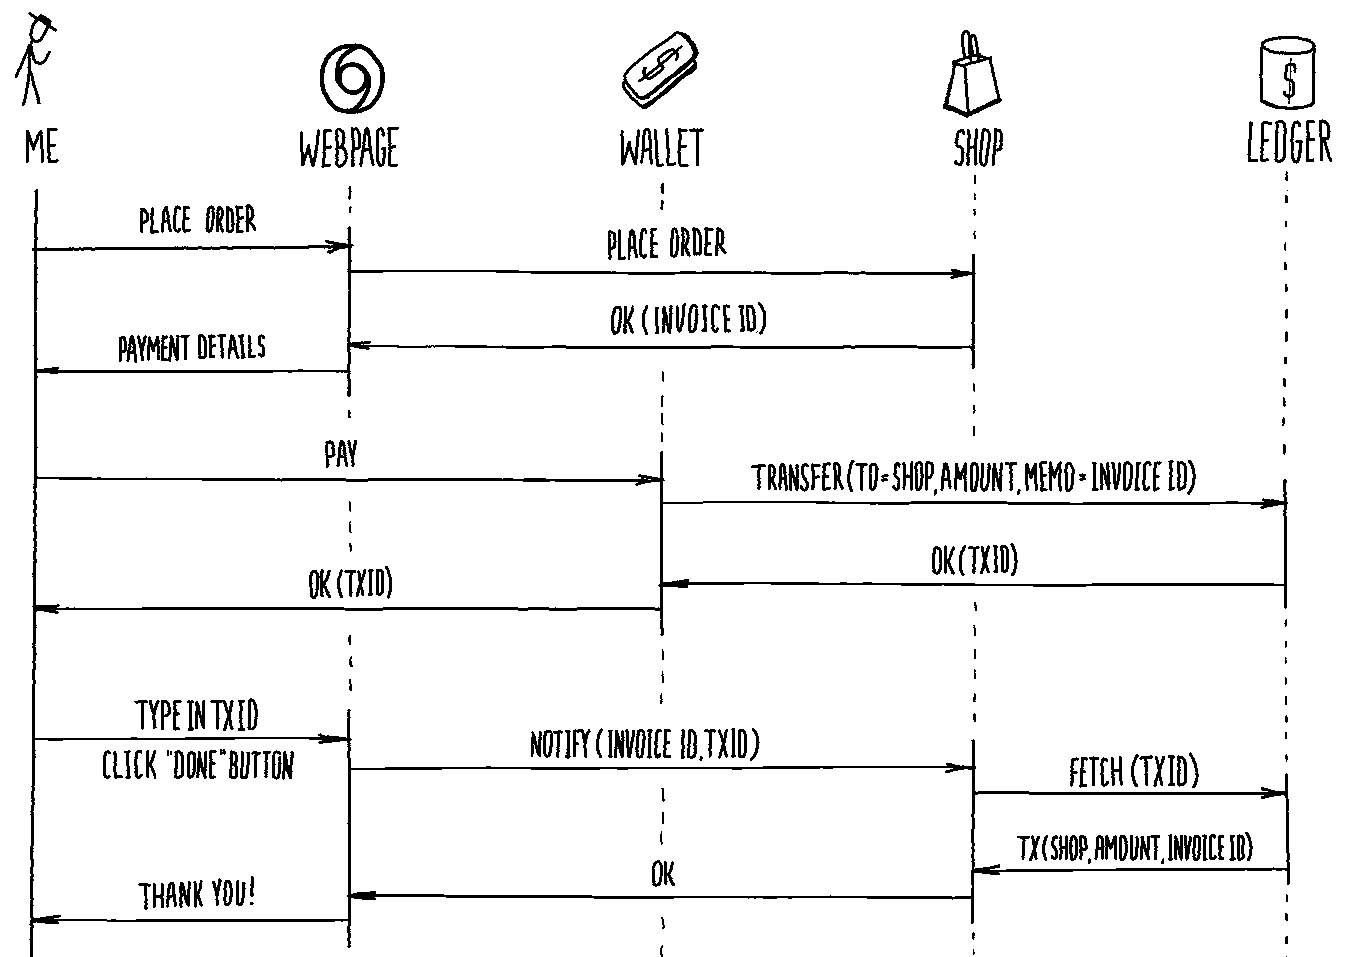
\includegraphics{/images/10-fetch-flow.png}
\end{figure}

\begin{itemize}
  \item The ledger must process at least two messages: a \code{transfer} from me and a \code{fetch} request from the shop.
  \item 
    The ledger charges one fee for my transfer.
    The transaction details are usually publicly available and require no access fee.
  \item The ledger does not need to store any additional information for the payment flow.
  \item The flow support unlimited concurrency.
  \item 
    Transaction access interfaces are handy and ubiquitous.
    Little additional complexity is usually required to enable the flow.
  \item 
    The failure cases are very similar to the \href{#invoice-account}{invoice-account} flow, except that there is no easy way to monitor outstanding invoices.
    One possible recovery is constructing an index of all the ledger transactions and scanning for transfers matching the open orders.
\end{itemize}

\section{conclusion}{Conclusion}

We analyzed several payment flows for ledgers hosted on the Internet Computer.
All the flows we discussed had \href{#payment-phases}{three phases}: negotiation, payment, and notification.

Below is a table comparing the payment flows.

\begin{tabular}{l l l l l}
 & \href{#invoice-account}{\normal{invoice account}} & \href{#approve-transfer-from}{\normal{approve-transfer-from}} & \href{#transfer-notify}{\normal{transfer-notify}} & \href{#transfer-fetch}{\normal{transfer-fetch}} \\
\hrule
Ledger messages & 2 & 2 & 2 & 2 \\
Fees & 2 & 2 & 1½ & 1 \\
Ledger memory (bytes) & 70 & 68 & 70 & 0 \\
Concurrent payments & \dingbat{heavy-check} & \dingbat{heavy-ballot-x} & \dingbat{heavy-check} & \dingbat{heavy-check} \\
Recurrent payments & \dingbat{heavy-ballot-x} & \dingbat{heavy-check} & \dingbat{heavy-ballot-x} & \dingbat{heavy-ballot-x} \\
Ledger complexity & simple & moderate & complex & simple \\
Failure recovery & not easy & ok & hard but rare & hard \\
\end{tabular}

So which flow is the best one?
None of them is a clear winner on all fronts.
You might prefer different flows based on your design goals and the application needs.
\end{document}
